\documentclass[10pt,a4paper,twoside]{article}
\usepackage[english]{babel}
%laad de pakketten nodig om wiskunde weer te geven :
\usepackage{amsmath,amssymb,amsfonts,textcomp}
%laad de pakketten voor figuren :
\usepackage{graphicx}
\usepackage{float,flafter}
\usepackage{hyperref}
\usepackage{inputenc}
\usepackage{minted}
\usepackage{subcaption}

\setlength\paperwidth{20.999cm}\setlength\paperheight{29.699cm}\setlength\voffset{-1in}\setlength\hoffset{-1in}\setlength\topmargin{1.499cm}\setlength\headheight{12pt}\setlength\headsep{0cm}\setlength\footskip{1.131cm}\setlength\textheight{25cm}\setlength\oddsidemargin{2.499cm}\setlength\textwidth{15.999cm}

\newcommand{\sweepsize}{0.26}

\begin{document}
\begin{center}
\hrule

\vspace{.4cm}
{\bf {\Huge Computer Vision} \\ {\huge Lab Assigment Report} \\ {\Large Local Features}}
\vspace{.2cm}
\end{center}
{\bf Tuan Mate Nguyen}  (tunguyen@student.ethz.ch)
\hrule



\section{Detection}
\subsection{Image gradients}

Computing the image gradients in the x and y direction, as described by 
\[ I_x(i,j) = \frac{I(i, j+1) - I(i,j-1)}{2}, I_y(i,j) = \frac{I(i+1, j) - I(i-1,j)}{2}\]
(where $i$ and $j$ are coordinates in the $y$ and $x$ direction, respectively) can be achieved by convolving the grayscale image with the following (1, 3) filter:
\begin{minted}[mathescape,
    linenos,
    numbersep=5pt,
    gobble=2,
    frame=lines,
    framesep=2mm,
    firstnumber=26]{csharp}
    dx = np.array([[-0.5, 0, 0.5]])
\end{minted}

In the y direction the kernel is just the transpose of the kernel for x
direction. In case the image has too much noise, the above filters could
be replaced with Sobel-filters (of the corresponding direction) which include some Gaussian blur.


\subsection{Local auto-correlation matrix}

Since $I_x(p')$ and $I_y(p')$ take the gradient values at $p'$ and then these values
are multiplied, we first need to do an element-wise multiplication of the image
gradients:
\begin{minted}[mathescape,
    linenos,
    numbersep=5pt,
    gobble=2,
    frame=lines,
    framesep=2mm,
    firstnumber=37]{csharp}
    Ix2 = Ix * Ix
    Iy2 = Iy * Iy
    Ixy = Ix * Iy
\end{minted}

Computing the weighted sum of the image gradient products in the neighbourhood of a
given pixel $p$ equals to applying a Gaussian blur on the image-gradient products:
\begin{minted}[mathescape,
    linenos,
    numbersep=5pt,
    gobble=2,
    frame=lines,
    framesep=2mm,
    firstnumber=43]{csharp}
    Gx2 = cv2.GaussianBlur(Ix2, ksize=ksize, sigmaX=sigma, borderType=cv2.BORDER_REPLICATE)
    Gy2 = cv2.GaussianBlur(Iy2, ksize=ksize, sigmaX=sigma, borderType=cv2.BORDER_REPLICATE)
    Gxy = cv2.GaussianBlur(Ixy, ksize=ksize, sigmaX=sigma, borderType=cv2.BORDER_REPLICATE)
\end{minted}

with the auto-correlation matrix being
\[M = \begin{bmatrix}
    Gx2 & Gxy\\ 
    Gxy & Gy2
  \end{bmatrix}\]

The kernel was set to $(0,0)$ so it's automatically set based on $\sigma$. 

%Here
%one could experiment with different blur kernel sizes, but it's worth mentioning
%that its size must not be bigger than the patch size, otherwise one
%could get wrong results due to the fact that then the blur kernel overlaps with
%the border padding. The padding values are always arbitrarily chosen (depending on the
%padding type) so their contribution to the sum is undesirable. 

\subsection{Harris response function}

Using the closed form formula from Harris $\&$ Stephens, the response function is 

\[C = det(M) - k trace^2(M)\]

which, using the previous results, yields

\begin{minted}[mathescape,
    linenos,
    numbersep=5pt,
    gobble=2,
    frame=lines,
    framesep=2mm,
    firstnumber=48]{csharp}
    C = Gx2*Gy2 - Gxy*Gxy - k * (Gx2 + Gy2)*(Gx2 + Gy2)
\end{minted}
Here $C$ is represented by a matrix where each element equals to the Harris-response
at the same position of the image (again, element-wise addition and
multiplication are needed).


%About Gaussian-blur: rotationally invariant hence better that simple box window\\
%compare results (number of detected keypoints)\\


\subsection{Detection criteria}

\subsubsection*{Common issues}
In all images the four corner points of the image are detected as false-positive corners. The
reason is that independently from border padding the pixel values will always
form a corner except when neighboring pixels have exactly the same value, which
is rare. However, later these will be filtered because they are too close to the
edges, so they won't cause problems. \par

The two most frequent problems of keypoints are ambiguity, meaning detecting
several keypoints for one actual corner, and detecting false positives in parts
where there is only an edge or even just a (noisy) flat area.


\subsubsection*{Parameter sweep}

\paragraph*{Threshold $T$:}

For $T=10^{-4}$ too few corners are detected, while for $T=10^-6$ too many (multiple keypoints for a single corner, keypoints along edges). As a result $T=10^{-5}$ was selected. 
\begin{figure}[h]
    \centering

    \begin{subfigure}{\sweepsize\textwidth}
    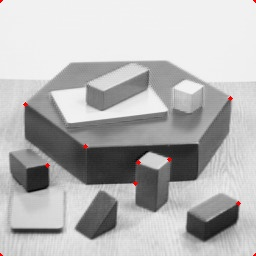
\includegraphics[width=0.9\linewidth, height=0.9\linewidth]{sweep_blocks/blocks_10_005_00001.jpg} 
    \caption{$T=10^{-4}$}
    \end{subfigure}
    \begin{subfigure}{\sweepsize\textwidth}
    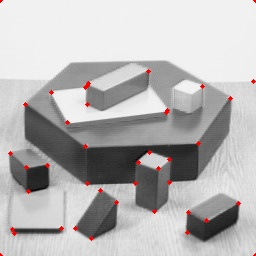
\includegraphics[width=0.9\linewidth, height=0.9\linewidth]{sweep_blocks/blocks_10_005_1e-05.jpg} 
    \caption{$T=10^{-5}$}
    \end{subfigure}
    \begin{subfigure}{\sweepsize\textwidth}
    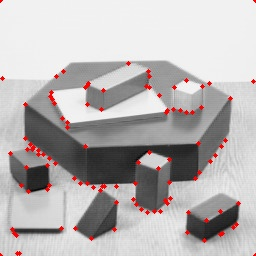
\includegraphics[width=0.9\linewidth, height=0.9\linewidth]{sweep_blocks/blocks_10_005_1e-06.jpg} 
    \caption{$T=10^{-6}$}
    \end{subfigure}
    
    \begin{subfigure}{\sweepsize\textwidth}
    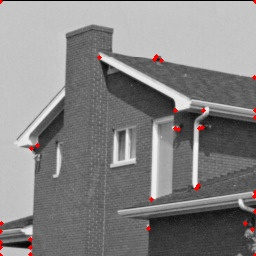
\includegraphics[width=0.9\linewidth, height=0.9\linewidth]{sweep_house/house_10_005_00001.jpg} 
    \caption{$T=10^{-4}$}
    \end{subfigure}
    \begin{subfigure}{\sweepsize\textwidth}
    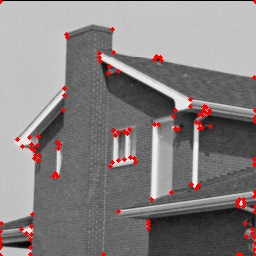
\includegraphics[width=0.9\linewidth, height=0.9\linewidth]{sweep_house/house_10_005_1e-05.jpg} 
    \caption{$T=10^{-5}$}
    \end{subfigure}
    \begin{subfigure}{\sweepsize\textwidth}
    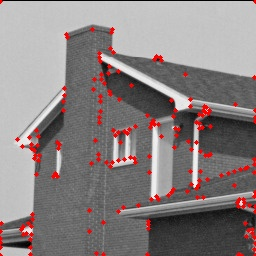
\includegraphics[width=0.9\linewidth, height=0.9\linewidth]{sweep_house/house_10_005_1e-06.jpg} 
    \caption{$T=10^{-6}$}
    \end{subfigure}
    \caption{Parameter sweep for $T$ with $\sigma=1.0$ and $k=0.05$}

\end{figure}

\paragraph*{Constant $k$:}

For different $k$ values there is not much difference between the obtained
keypoints. In general a lower $k$ value results in slightly more detected
keypoints, however, sometimes among these are a few that don't correspond to
corners or several keypoints are present for the same corner. For further experiments $k=0.05$ was used.
\begin{figure}[h]
    \centering

    \begin{subfigure}{\sweepsize\textwidth}
    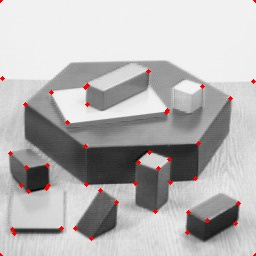
\includegraphics[width=0.9\linewidth, height=0.9\linewidth]{sweep_blocks/blocks_10_004_1e-05.jpg} 
    \caption{$T=0.04$}
    \end{subfigure}
    \begin{subfigure}{\sweepsize\textwidth}
    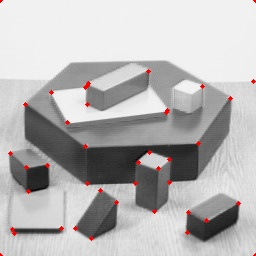
\includegraphics[width=0.9\linewidth, height=0.9\linewidth]{sweep_blocks/blocks_10_005_1e-05.jpg} 
    \caption{$T=0.05$}
    \end{subfigure}
    \begin{subfigure}{\sweepsize\textwidth}
    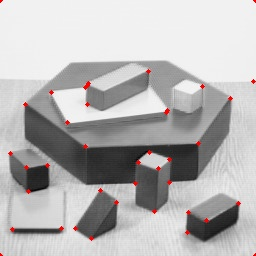
\includegraphics[width=0.9\linewidth, height=0.9\linewidth]{sweep_blocks/blocks_10_006_1e-05.jpg} 
    \caption{$T=0.06$}
    \end{subfigure}
    
    \begin{subfigure}{\sweepsize\textwidth}
    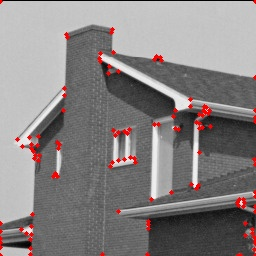
\includegraphics[width=0.9\linewidth, height=0.9\linewidth]{sweep_house/house_10_004_1e-05.jpg} 
    \caption{$T=0.04$}
    \end{subfigure}
    \begin{subfigure}{\sweepsize\textwidth}
    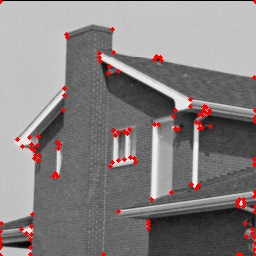
\includegraphics[width=0.9\linewidth, height=0.9\linewidth]{sweep_house/house_10_005_1e-05.jpg} 
    \caption{$T=0.05$}
    \end{subfigure}
    \begin{subfigure}{\sweepsize\textwidth}
    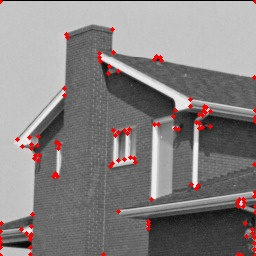
\includegraphics[width=0.9\linewidth, height=0.9\linewidth]{sweep_house/house_10_006_1e-05.jpg} 
    \caption{$k=0.06$}
    \end{subfigure}
    \caption{Parameter sweep for $k$ with $\sigma=1.0$ and $T=10^{-5}$}

\end{figure}

\paragraph*{Standard deviation $\sigma$:}

With small ($\sigma=0.5$) standard deviation obvious corners are missed (see
blocks image). Applying bigger blur ($\sigma=1.0$) gives more points but these
are often redundant. The best result is achieved with $\sigma=2.0$, which
detects most of the sharp corners while avoiding duplicate keypoints.
\begin{figure}[h]
    \centering

    \begin{subfigure}{0.25\textwidth}
    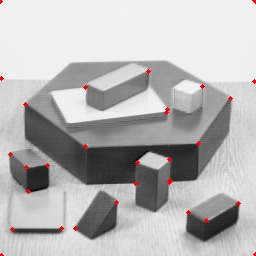
\includegraphics[width=0.9\linewidth, height=0.9\linewidth]{sweep_blocks/blocks_05_005_1e-05.jpg} 
    \caption{$\sigma=0.5$}
    \end{subfigure}
    \begin{subfigure}{0.25\textwidth}
    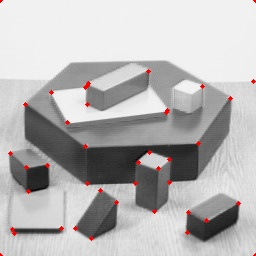
\includegraphics[width=0.9\linewidth, height=0.9\linewidth]{sweep_blocks/blocks_10_005_1e-05.jpg} 
    \caption{$\sigma=1.0$}
    \end{subfigure}
    \begin{subfigure}{0.25\textwidth}
    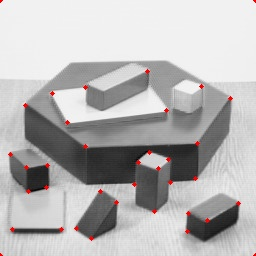
\includegraphics[width=0.9\linewidth, height=0.9\linewidth]{sweep_blocks/blocks_20_005_1e-05.jpg} 
    \caption{$\sigma=2.0$}
    \end{subfigure}
    
    \begin{subfigure}{0.25\textwidth}
    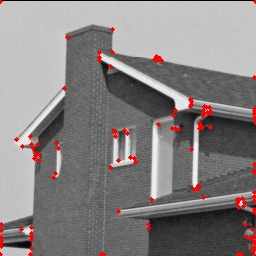
\includegraphics[width=0.9\linewidth, height=0.9\linewidth]{sweep_house/house_05_005_1e-05.jpg} 
    \caption{$\sigma=0.5$}
    \end{subfigure}
    \begin{subfigure}{0.25\textwidth}
    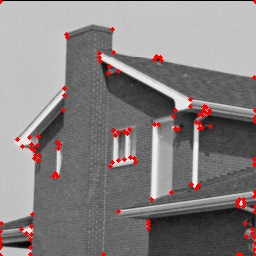
\includegraphics[width=0.9\linewidth, height=0.9\linewidth]{sweep_house/house_10_005_1e-05.jpg} 
    \caption{$\sigma=1.0$}
    \end{subfigure}
    \begin{subfigure}{0.25\textwidth}
    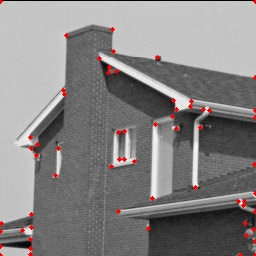
\includegraphics[width=0.9\linewidth, height=0.9\linewidth]{sweep_house/house_20_005_1e-05.jpg} 
    \caption{$\sigma=2.0$}
    \end{subfigure}
    \caption{Parameter sweep for $\sigma$ with $k=0.05$ and $T=10^{-5}$}

\end{figure}

\clearpage

\section{Description and matching}
\subsection{Local descriptors}

Patches are centered around the keypoint so they need to have an odd pixel size.
\begin{minted}[mathescape,
    linenos,
    numbersep=5pt,
    gobble=2,
    frame=lines,
    framesep=2mm,
    firstnumber=8]{csharp}
    assert(patch_size % 2 == 1)
\end{minted}

Only those keypoints are kept that are at least half patch-size pixel away from
the edges in both direction. The accepted area is a subrectangle with the
following top-left and bottom-right coordinates:

\begin{minted}[mathescape,
    linenos,
    numbersep=5pt,
    gobble=2,
    frame=lines,
    framesep=2mm,
    firstnumber=11]{csharp}
    d = patch_size // 2 

    height, width = img.shape
    # Points' coordinates must be "min. distance" far away from both edges,
    # along both axises
    min_w_idx = min_h_idx = d
    max_w_idx = (width-1)-d
    max_h_idx = (height-1)-d

    # These intervals define a sub-rectangle in the image, with the following
    # top-left/bottom-right coordinates:
    tl = np.array([min_w_idx, min_h_idx])
    br = np.array([max_w_idx, max_h_idx])

\end{minted}

\subsection{Sum of squared differences - one way}

In order to be able to iterate through features of all pairs of keypoints, a
meshgrid is first created for their indices. This just contains coordinates of a 2-D mesh where
each coordinate will correspond to a keypoint index from the first and second
image. The result are two 2-D arrays containing these "index coordinates" of the mesh.
\begin{minted}[mathescape,
    linenos,
    numbersep=5pt,
    gobble=2,
    frame=lines,
    framesep=2mm,
    firstnumber=20]{csharp}
    grid_idx1, grid_idx2 = np.meshgrid(idx1, idx2, indexing='ij')
\end{minted}

The SSD can then simply be computed in a vectorized way:
\begin{minted}[mathescape,
    linenos,
    numbersep=5pt,
    gobble=2,
    frame=lines,
    framesep=2mm,
    firstnumber=24]{csharp}
    ssd = np.sum(np.square(desc1[grid_idx1,:] - desc2[grid_idx2,:]), -1)
\end{minted}

For the one-way nearest neighbor matching first an array is created with the
keypoint indices of from the first image. Then for each of them, the SSDs from
the comparison with descriptors from the second image are sorted in ascending
order. The smallest SSD will define mathcing keypoints.
\begin{minted}[mathescape,
    linenos,
    numbersep=5pt,
    gobble=2,
    frame=lines,
    framesep=2mm,
    firstnumber=45]{csharp}
        x = np.arange(q1)
        y = np.argmin(distances, 1)
        matches = np.array([x, y]).transpose()
\end{minted}

\begin{figure}[t]
    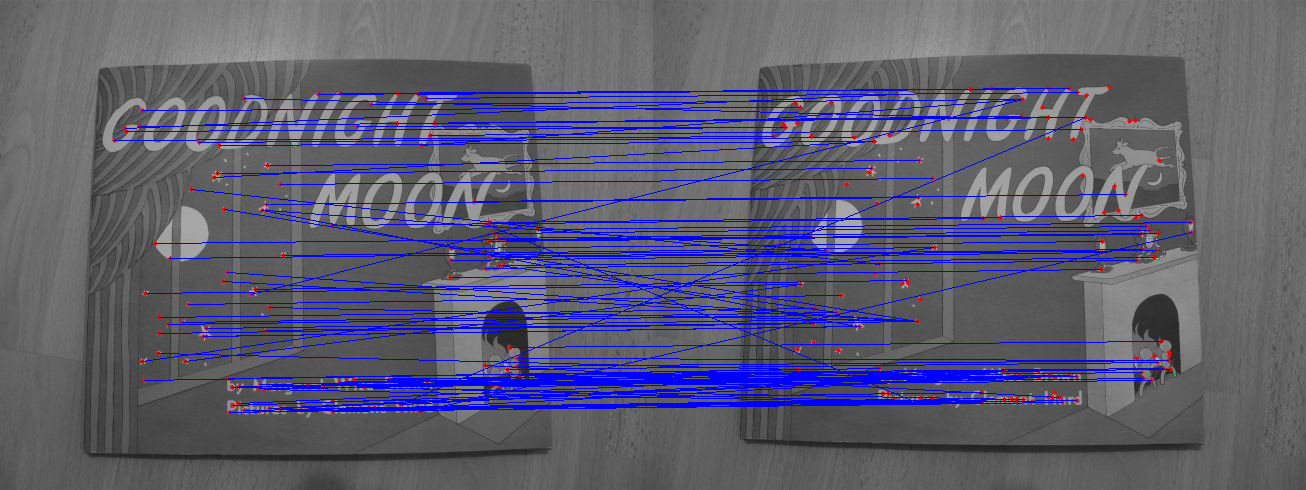
\includegraphics[width=\textwidth]{match_ow.png}
    \centering
    \caption{Matching keypoints for one-way nearest neighbor matching}
    \label{match_ow}
\end{figure}

As it can be seen in Fig.\ref{match_ow}, all keypoints from the first image
match with some points from the second. On the other hand in the second image
some keypoints are left unpaired. It is worth mentioning that this would be the
case even if the two images would be completely different. An inherent flaw of
this approach is that the corresponances can have many-to-one relation ship,
resulting in ambiguity. This can happen if several descriptors from the first
image are closest to the same descriptor from the second image. These have to be
filtered out, otherwise the homography cannot be determined.

\subsection*{Mutual nearest neighbors} 
One solution is to verify the closest descriptor from the other image's
perspective as well. The mutual proximity can be checked by getting each
keypoint (in the first image) $x1$'s nearest neighbor (in the second image)  $y1$'s nearest
neighbor (in the first image) $x2$. If this is the same as the original keypoint,
they match:
\begin{minted}[mathescape,
    linenos,
    numbersep=5pt,
    gobble=2,
    frame=lines,
    framesep=2mm,
    firstnumber=57]{csharp}
    x2 = np.argmin(distances, 0)
    x = x1[np.where(x1 == x2[y1])]
\end{minted}


Mutual matches guarantee one-to-one relationships. A
consequence is that now a match is not guaranteed for all keypoints in either
images (in theory one could end up without having any matches). This is nicely
shown in Fig.\ref{match_mutual}. The quality of the matching is higher compared
to the one-way matching, since not every keypoints are forced to have a pair,
only those that are good matches, meaning being mutually close.

\begin{figure}[H]
    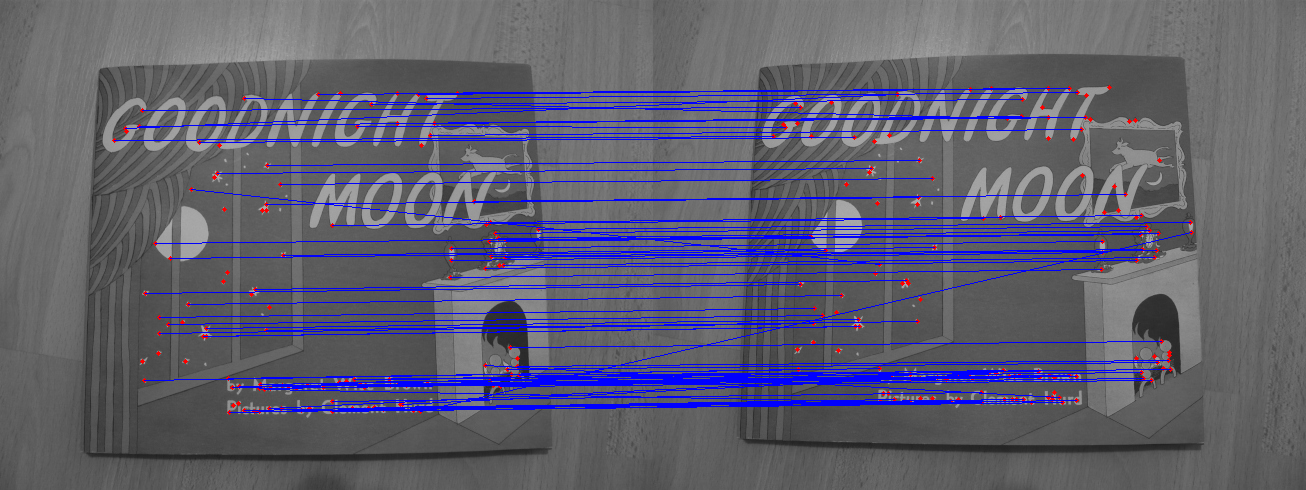
\includegraphics[width=\textwidth]{match_mutual.png}
    \centering
    \caption{Matching keypoints for mutual nearest neighbor matching}
    \label{match_mutual}
\end{figure}

For the ratio test matching, we partially sort (with $np.partition$) the SSDs from
the comparison with descriptors from the second image, so that the first two
elements - (0,1) - in every row are the nearest and second nearest neighbors. 

\begin{minted}[mathescape,
    linenos,
    numbersep=5pt,
    gobble=2,
    frame=lines,
    framesep=2mm,
    firstnumber=68]{csharp}
        closest_matches = np.partition(distances, (0,1), 1)
\end{minted}
When
dividing, we also must ensure that the second SSD is not zero. This can be the
case when the second image contains two or more features that are bitwise
identical to one in the first image (for example synthetic image with repetitive
patterns). In this case the value can be set to np.nan and be ignored
because the match would be ambiguous anyway.

Their ratio are then thresholded to find the final matches:
\begin{minted}[mathescape,
    linenos,
    numbersep=5pt,
    gobble=2,
    frame=lines,
    framesep=2mm,
    firstnumber=75]{csharp}
        x = np.where((~np.isnan(closest_matches[:,1])) & 
                     (closest_matches[:, 0]/closest_matches[:, 1] < ratio_thresh))[0]
        y = np.argmin(distances, 1)[x]
        matches = np.array([x, y]).transpose()
\end{minted}

Since the thresholding criteria doesn't necessarily hold, there are again
unpaired keypoints. There are also fewer matches, as the requirement for
sufficiently distinctive features further eliminates candidates.

\begin{figure}[H]
    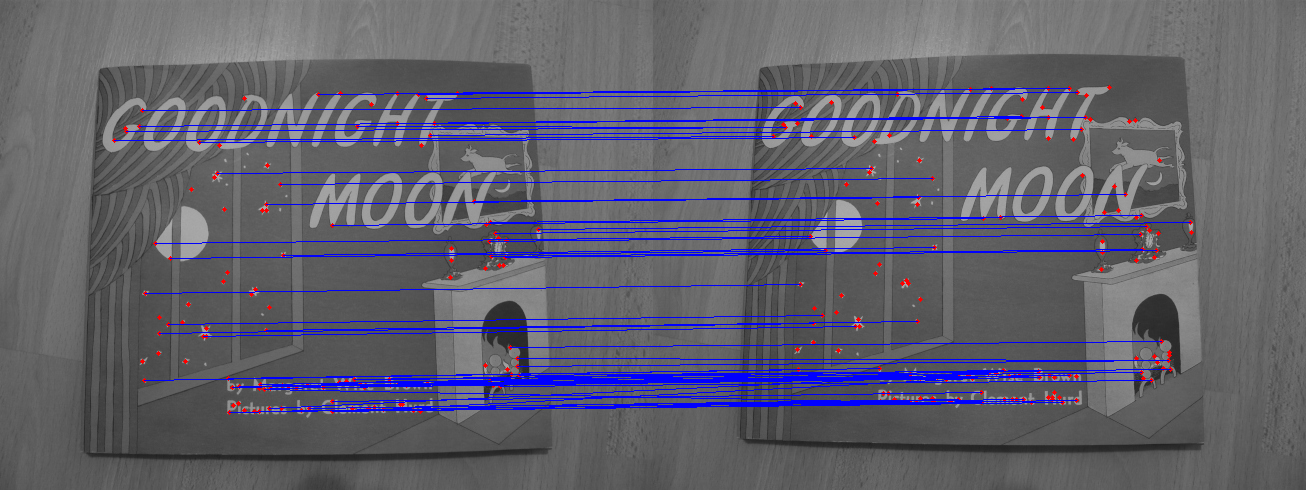
\includegraphics[width=\textwidth]{match_ratio.png}
    \centering
    \caption{Matching keypoints for ratio test matching}
    \label{match_ratio}
\end{figure}

\end{document}
